\documentclass[conference]{IEEEtran}

\usepackage[linesnumbered,ruled,vlined]{algorithm2e}
\usepackage{multirow}
\usepackage{amsmath,amsthm}
\usepackage{amssymb}
\usepackage{fixltx2e}
\usepackage{enumerate}
\usepackage{graphicx,subfigure}
\usepackage{url}

\newtheorem{theorem}{Theorem}
\newtheorem{problem}{Problem}
\newtheorem{definition}{Definition}

\begin{document} 

\title{QoS-Guaranteed Controller Placement in SDN}
\author{\IEEEauthorblockN{Tracy Y. Cheng, Mengqing Wang, Xiaohua Jia}
\IEEEauthorblockA{City University of Hong Kong\\
Email: \{tracy.cheng, mengq.wang\}@my.cityu.edu.hk, csjia@cityu.edu.hk}}
\maketitle

\begin{abstract}
The controller placement problem tries to place $k$ controllers in a given network to optimize performance metrics such as propagation latency, load distribution, network reliability and failure resilience. However, the quality of service (QoS) is always a primary concern of the network operators in the placement of SDN controllers. Since the SDN controllers are responsible to provide services for routers, the response time of controllers is an important QoS parameter of network operators. In this paper, we introduce the QoS-Guaranteed Controller Placement problem: Given a network topology and a response time bound, how many controllers are needed, where to place them, and which routers are assigned to each of the controller. We propose three heuristic algorithms: incremental greedy algorithm, primal-dual-based algorithm and network-partition-based algorithm. The proposed algorithms are tested and compared on the Internet Topology Zoo, a dataset of public available network topologies. Simulation results show that the proposed three methods have the similar performance on all input topologies. 
\end{abstract}

\begin{IEEEkeywords}
Software-Defined Networks, Controller Placement, QoS Guaranteed.
\end{IEEEkeywords}

\section{Introduction}

The software-defined network (SDN) aims to decouple the control plane from the data plane \cite{nunes2014survey}. It uses the network controller to control the routing behavior of routers or switches, so routers can focus on data forwarding. In a wide area network (WAN), it requires multiple physically dispersed controllers in the network, each of which manages and operates the routers in its local area. There are some works regarding the design and implementation of distributed systems of SDN controllers, such as ElastiCon \cite{dixit2013towards}, Onix \cite{koponen2010onix} and HyperFlow \cite{tootoonchian2010hyperflow}. 

In the design of distributed control plane, the location of controllers has significant impact on the network performance. There are two major factors that affect the performance of controllers: 1) the network distance between routers and controllers. In a WAN, the network delay between a router to its controller becomes non-negligible and this delay affects the response time of controllers \cite{jain2013b4}. 2) load balancing among the controllers. Some controller could be overloaded while others are less busy. Therefore, it is an important research topic to place controllers properly in a network.       

The controller placement problem has been studied in recent years. Heller et al. first introduced the controller placement problem in \cite{heller2012controller}. The problem is to place $k$ controllers in a given network such that the propagation delay between routers to controllers is minimized. Several follow up works focused on the optimization of other performance metrics for placing $k$ controllers in a network \cite{schmid2013exploiting,jimenez2014controller,yao2014capacitated,ros2014five,hock2013pareto}. 
The work in \cite{schmid2013exploiting} aims to minimize the communication delay between controllers. Load distribution among controllers is considered in \cite{jimenez2014controller}. The controller capacity is considered in \cite{yao2014capacitated}, the network reliability is considered in \cite{ros2014five}, failure resilience is considered in \cite{hock2013pareto}, etc. 

However, the issues of minimizing the number of controllers and the quality of service (QoS) have not been considered in the previous work. In network design, QoS is always a primary concern of the network operators in the placement of SDN controllers. Since the SDN controllers are responsible to provide services for routers to setup routing information of traffic flows, the response time of controllers is an important QoS parameter for network operations. The response time of a controller consists of two components: 1) the round trip of network delay between the controller and a router, and 2) the service time of the controller, which depends on the service capacity and the work load of the controller. 

In this paper, we study the QoS guaranteed controller placement problem, which is to place the minimum number of controllers in the network such that response time of controllers can meet a given delay bound. That is, given a delay bound, we need to determine: a) how many controllers are needed, b) where to place them, c) which routers are assigned to each of the controllers. This problem is more complicated than the traditional controller placement problems that were studied in the literatures. This is because the response time considered in our problem includes the service time of the controllers, which depends on the workload of the controllers. The traditional optimization methods for k-median or k-center problems are not applicable to our problem.

For the proposed QoS-guaranteed controller placement problem, we propose three heuristic algorithms: incremental greedy algorithm, primal-dual-based algorithm and network-partition-based algorithm. Extensive simulations have been done to compare the performance of the three heuristic algorithms on the same dataset. The simulations are performed on the Internet Topology Zoo \cite{knight2011internet}, which is a database including publicly available network topologies. The simulation results show that the three methods have the similar performance on all input topologies. 

The remining of the paper is organized as follows: Section \ref{sec:relatedwork} presents the related work on the controller placement problem in SDN. Section \ref{sec:model} gives the system model and problem formulation. Section \ref{sec:solution} introduces our solutions. Section \ref{sec:simulation} shows the simulation and related analysis. Finally conclusion is given in \ref{sec:conclusion}.

\section{Related Work}
\label{sec:relatedwork}

To address the controller placement problem, there are some research works considering different performance metrics such as node-to-controller latency \cite{heller2012controller}, network reliability \cite{ros2014five}, load of controllers \cite{yao2014capacitated}, inter-controller delay \cite{jimenez2014controller}, failure resilience \cite{hock2013pareto}, etc.

The controller placement problem was firstly introduced by \cite{heller2012controller}. This work aims to minimize the average latency between controllers and routers. It is pointed out that the average latency and the maximal latency cannot be optimized at the same time, and a K-means greedy method was employed to find the optimal placement that minimizes the average latency and k-center greedy method was proposed to minimize the maximal latency. 

A fault tolerant controller placement was proposed in \cite{ros2014five}. The author formulated the fault tolerant controller problem considering the network reliability constraint. A heuristic algorithm was proposed to computes placements with the required reliability. This work concludes that each node is required to connect to 2 or 3 controllers, which typically provide more than five nines reliability.

The load of controllers is taken into account for designing controller placement in \cite{yao2014capacitated}. The controller problem was extended to a capacitated problem where there is an upper bound for the load of each controller. The author proposed a greedy K-center algorithm to solve the problem.

The propagation delay among controllers is taken into consider in \cite{jimenez2014controller} for designing the control plane. A K-critical algorithm is developed to find the minimum number of controllers to satisfy a target communication between controllers and nodes, such as delay, latency, convergence time, etc.

Failure resilience is considered in \cite{hock2013pareto} for placing controllers. This work concludes that whereas one controller is enough from a latency point-of-view, more controllers are needed to meet resilience requirement. They also consider inter-controller latency, load balancing between controllers, and trade-off considerations between latency and failure resilience. A framework for resilience pareto-based optimal controller placement is proposed that provides network operators with all pareto-optimal requirements. 

The previous works on the controller placement problem focus on placing a given number of controllers to optimize a given performance metric such as propagation delay, controller load distribution, network reliability, etc. However, minimizing the number of controllers has not been considered and the QoS has not been guaranteed in the previous work. The response time of the request sent from a router to its controller is an important parameter of QoS. Therefore, we propose the QoS-guaranteed controller placement problem to determine: 1) the minimal number of controllers needed; 2) where to place them; 3) which router is under controller of each of them.     
 

\section{System Model and Problem Formulation}
\label{sec:model}

In this section, we first formulate the response time of a request from a router to a controller, which is performance metric considered in our controller placement problem. Then we formulate the proposed QoS-guaranteed controller placement problem.

The network is modeled by graph $G(V, E)$, where $V$ represents network routers, $E$ represents the network links between nodes. Each router $i\in V$ is associated with a request demand $r_i$. Each router's location is also a candidate site for placing a controller. Suppose all controllers have the same processing capacity $\mu$. Our goal is to find the minimal subset $C\in V$ to place a controller in each node of $C$, such that the QoS requirement is met.    

\begin{table}
\caption{Notations}
\label{table:notations}
\centering
\begin{tabular}{|c|l|}
\hline Notation & \multicolumn{1}{|c|}{Meaning} \\
\hline $V$ & set of routers \\
\hline $C$ & set of controllers \\
\hline $\delta$ & upper bound of response time\\
\hline $r_i$ & the requesting rate of router $i$ \\
\hline $t_i$ & response time of request from router $i$ \\
\hline \rule{0pt}{0.3cm} $\bar{t}$ & average response time of all routers \\
\hline $\mu$ & service capacity of each controller \\
\hline $\lambda_j$ & traffic arrival rate of controller $j$ \\
\hline $\tau_j$ & mean service time of controller $j$ \\
\hline $S_j$ & serving range of controller $j$ \\
\hline $x_{ij}$ & variable indicates whether router $i$ is assigned to controller $j$ \\
\hline $y_j$ & variable indicates whether controller candidate $j$ is open \\
\hline $a_j$ & variable indicates whether set $S_j$ is selected \\
\hline $b_i$ & dual variable of router $i$ \\
\hline
\end{tabular}
\end{table}

The main job of a controller in SDN is to set up routing information for flows upon request from routers \cite{tootoonchian2012controller}. The flow setup process works as follows: When the first packet of a new flow arrives at an OpenFlow switch, its header information is extracted and then matched against the flow table entries. If there is no match found for the packet, the packet is forwarded to the controller for processing. The controller will send the routing information to the router to help set up the flow table for the new flow of this packet \cite{sezer2013we}. The response time of a request sent from a router is defined as the time from the moment of sending out this request until the reply is received from its controller. Given a upper bound $\delta$ of the response time, our task is to place the minimum number of controllers in $V$ such that the average response time for all routers is within the given bound $\delta$. 

We introduce two variables, $X$ and $Y$, to respectively denote the assignment of routers to controllers and the placement of controllers. For router $i$ and controller $j$, $x_{ij}=1$ if router $i$ is assigned to controller $j$ and $x_{ij}=0$ otherwise; $y_j=1$ if there is a controller placed at node $j$ and $y_j=0$ otherwise. 
The response time of a flow setup request from a router has two components: 1) the round trip time from the switch to its controller, and 2) the service time of the controller for the request. We first take a look at the service time of a controller.       

Each controller can be modeled as a M/M/1 queueing model. Suppose packets arrive according to a Poisson process and the processing times of the packets are independent and identically exponentially distributed. Let $\lambda_j$ denote the total arrival rate of packets at the controller $j$, which is represented as:
\begin{equation}
\lambda_j = \sum_{\forall i\in S} r_ix_{ij},
\end{equation}
where $r_i$ is the request rate of router $i$. 

The packets in one controller are processed according to First-Come-First-Serve order. Each controller $j\in V$can only accept number of clients within its capacity $\mu$, therefore it is required that: $\lambda_j<\mu$.


According to the queueing theory \cite{gross2008fundamentals}, the expected mean service time of controller $j$ is defined as:
\begin{equation}
\begin{aligned}
\tau_j & = \frac{1}{\mu-\lambda_j} \\
& = \frac{1}{\mu-\sum_{i} r_ix_{ij}}
\end{aligned}
\end{equation}

For each router $i$, let $t_i$ denote the response time of its request, which can be represented as:
\begin{equation}
\begin{aligned}
t_i & = 2t_{ij}+\tau_j \\
& = 2t_{ij}+\frac{1}{\mu-\sum_{i}r_ix_{ij}},
\end{aligned}
\end{equation}
where $t_{ij}$ denotes the network delay between router $i$ and controller $j$. We assume the request and reply between the router and the controller always take the shortest path in the network. $t_{ij}$ is the sum of the link delay of the shortest path between nodes $i$ and $j$ in the network.

Let $\bar{t}$ denote the mean response time, which is defined as:
\begin{equation}
\bar{t}=\frac{1}{|R|}\sum_{i\in R}t_i
\end{equation}

In this paper, we define the QoS-guaranteed controller placement problem as follows:
\begin{definition}
Given a network topology $G$, we are asked to place the minimal number of controllers subject to the response time constraint: $\bar{t}\leq \delta$. 
\end{definition}

\section{Heuristic Algorithm}
\label{sec:solution}

Each router's location is a candidate site for placing a controller. We compute the service range of each candidate site. The service range of a candidate site include all routers whose requests have a response time less than or equal to $\delta$ from this controller candidate, which guarantees the QoS requirement. Let $S_j$ denote the set of routers within the service range of candidate site $j\in V$. Our proposed QoS-guaranteed controller placement problem can be described as: Given a set $V$ of $n$ routers, a collection of subsets of $V$: $S=\{S_1, ..., S_n\}$, find a minimum subcollection of $S$ that serves all routers of $V$. To solve this problem, we design and compare three heuristic algorithms: incremental greedy algorithm, primal-dual-based algorithm and network-partition-based algorithm.


\subsection{Incremental Greedy Algorithm}
The incremental greedy algorithm iteratively picks the largest set and removes the served routers. In each iteration, open the controller candidate $j$ associated with the selected set $S_j$. Routers within the set $S_j$ are assigned to this controller $j$. This iteration is repeated until every router is served by one controller.   

The detail of greedy algorithm is illustrated in Algorithm \ref{alg:naive}. At the begining, we compute the service range of each candidate site. Suppose each candidate site is placed with a controller, the service range of a cadidate site include all routers whose requests have a response time less than or equal to $\delta$ from the controller at this candidate site. In each iteration, the candidate site with the largest service range is chosen to place a controller. Unserved routers within its service range are assigned to this controller. This iteration is repeated until all routers are being served. 

\begin{algorithm}[!htbp]
%\DontPrintSemicolon % Some LaTeX compilers require you to use \dontprintsemicolon instead 
\KwIn{Graph $G=(V, E)$, Response time bound $\delta$;}
\KwOut{$X, Y$;}
\BlankLine
$R\leftarrow V$, $C\leftarrow V$ \;
$y_j=0, \ \forall j\in C$ \;
$x_{ij}=0, \ \forall i\in R, j\in C$ \;
\While{$R\neq \emptyset$}{	
	\ForEach{$j\in C$} {				
		Compute the service range of candidate site $j$\;
		}	
	Find candidate site $j$ which has the largest service range and set $y_j=1$\;
	$C\leftarrow C-\{j\}$ \;
	\ForEach{router $i$ within the service range of $j$}{
		$x_{ij}=1$ \;
		$R\leftarrow R-\{i\}$ \;
	}
	
}		
\Return $X, Y$
\caption{Incremental Greedy Algorithm}
\label{alg:naive}
\end{algorithm}

\subsection{Primal-Dual-based Algorithm}

The incremental greedy algorithm does not have a performance guarantee for all kinds of inputs. It's performance often varies on different input. The primal-dual schema is used for designing approximation algorithms for integer programming problems, which provides a approximation ratio compared with the optimal solution. The basic idea is to consider the LP-relaxation of the original integer program as the primal program. We derive the dual program of the primal program. Then we settle down the complementary slackness condition of the primal program and the dual program respectively. In the primal-dual schema, we start with initial feasible solutions to the primal and dual programs, it iteratively starts satisfying complementary slackness conditions. The current primal solution is used to determine the improvement to the dual solution, and vice versa. This algorithm is ended when a primal feasible solution is obtained and all complementary slackness conditions are satisfied.

To formulate the proposed controller placement problem as an integer program, let us assign a variable $a_j$ for each set $S_j\in S$, which is allowed to be 0/1 values. The set $S_j$ represents the set of routers within the service range of controller candidate $j$. $a_j$ is set to 1 iff set $S_j$ is selected, 0 otherwise. For each router $i\in V$, it is required that at least one of the sets containing it be selected. The controller placement problem can be formulated as:
\rule{0.5\textwidth}{0.5pt}
\begin{equation}
\begin{aligned}
& \text{minimize} & & \sum_{S_j\in S}a_j \\
& \text{subject to} & &  \sum_{S_j: i\in S_j}a_j \ge 1, \quad & \forall i\in V \\
& & & a_j\in \{0,1\}, \quad & \forall j\in V
\end{aligned}
\end{equation}
\rule{0.5\textwidth}{0.5pt}

The LP-relaxation of this integer program is obtained by letting the domain of variables $a_j$ be $a_j\ge 0$, which is the primal program. We introduce a variable $b_i$ for each router $i\in V$, we obtain the dual program.
\rule{0.5\textwidth}{0.5pt}
\begin{equation}
\begin{aligned}
& \text{minimize} & & \sum_{i\in V}b_i \\
& \text{subject to} & &  \sum_{i: i\in S_j}b_i \leq 1, \quad & \forall S_j\in S \\
& & & b_i\ge 0, \quad & \forall i\in V
\end{aligned}
\end{equation}
\rule{0.5\textwidth}{0.5pt}

The complementary slackness conditions are:
\begin{equation}
\begin{aligned}
& \text{Primal condition:} & & a_j\ne 0 \Rightarrow \sum_{i: i\in S_j}b_i=1, \ \forall S_j\in S\\
& \text{Dual condition:} & & b_i\ne 0 \Rightarrow \sum_{S_j: i\in S_j}a_j\leq f, \ \forall i\in V 
\end{aligned}
\end{equation}
Define the frequency of an router to be the number of sets it is in. $f$ denotes the frequency of the most frequent router. Set $S_j$ is said to be tight if $\sum_{i: i\in S_j}b_i=1$. The primal variable $a_j$ is incremented integrally, which means to pick only tight sets in the system. 

The primal-dual algorithm proceeds in iterations. In each iteration, we pick an unserved router, say $i$, and raise $b_i$ until some set goes tight. Pick all tight sets and open the related controller candidates. For each tight set, assign routers within the set to the related controller. For routers covered by multiple tight sets, each of them can randomly choose a tight set and connect to its controller. Then the unselected sets and unserved routers are updated. This iteration is repeated until all routers are served. This primal-dual algorithm achieves an approximation factor of $f$. The detail of this primal-dual algorithm is illustrated in Algorithm \ref{alg:primal-dual}.

To help illustrate this primal-dual-based controller placement algorithm, we give an example. In Figure \ref{fig:example}, there are some sets $\{N_1, N_{13}\}$, $\{N_2, N_{13}\}$, $\{N_3, N_{13}\}$, ... $\{N_9, N_{13}\}$, $\{N_{21}, N_{22}\}$. Each of these sets represents a service range of a controller candidate. Suppose the algorithm raises $b_{13}$ in the first iteration. When $b_{13}$ is raised to 1, all sets including $N_{13}$ go tight. They are all picked in the system, thus routers $N_1, N_2, N_3, ..., N_9$ are served by the controllers of the tight sets. In the second iteration, $b_{21}$ is raised to 1 and the set $\{N_{21}, N_{22}\}$ goes tight. Pick the set  $\{N_{21}, N_{22}\}$ into the system and all routers are being served by at least one controller. 

\begin{figure}[!htbp]
\center
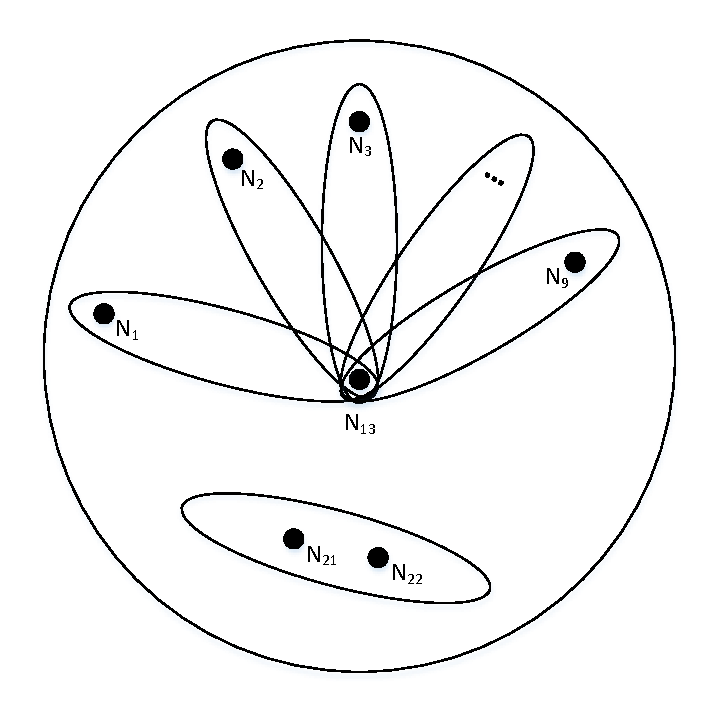
\includegraphics[width=0.4\textwidth]{fig/set-cover.pdf}
\caption{An expample of applying primal-dual-based algorithm}
\label{fig:example}
\end{figure}

\begin{algorithm}[!htbp]
%\DontPrintSemicolon % Some LaTeX compilers require you to use \dontprintsemicolon instead 
\KwIn{Graph $G=(V, E)$, Response time bound $\delta$;}
\KwOut{$X, Y$;}
\BlankLine
\ForEach{$j\in V$}{
	compute the service range and $S_j$ \;
}
$S=\{S_j, \forall j\in V\}$ \;
$a_j=0, \ \forall j\in S$ \;
$b_i=0, \ \forall i\in V$ \;
\While{$V\ne \emptyset$}{
	Pick an unserved router, say $i$, and set $b_i\leftarrow b_i+1$;
	Find all sets that go tight \;
	\ForEach{tight $S_j$}{
		Set $a_j=1$ and open the controller $j$ \;
		Assign all routers within $S_j$ to controller $j$ \;
		$V\leftarrow V-\{i|i\in S_j \}$ \;
	}
}
\Return $X, Y$
\caption{Primal-Dual-based Algorithm}
\label{alg:primal-dual}
\end{algorithm}

\subsection{Network-Partition-based Algorithm}
The above greedy algorithm and the primal-dual algorithm don't have a global view of the whole network. They create unbalanced placement and unbalanced load among controllers. Next we design a network-partition-based algorithm which considers the load balancing among all controllers. 

The basic idea of network-partition-based method is to divide the network into partitions and place controllers in each partition seperately. First, the network is divided into partitions. In each partition, the largest propagation delay between any two routers is equal to the bound $\delta$. In each partition, we use the incremental greedy method to place controllers. Since we limit the service range of each controller to one partition, the load distribution among all controllers is balanced.

The detail of the network-partition-based algorithm is described in Algorithm \ref{alg:divide}. First, the network is divided into grids. Any pair of routers within each grid has a communication delay less than $\delta$.
In the network partitioning, we first divide the network into vertical strips, where each strip is left closed and right open. In each strip, the propagation delay between the node on the left boundary and the node on the right boundary is equal to $\delta$. Then each strip is divided into grids. In each grid, the propagation delay between the node on the top boundary and the node on the bottom boundary is equal to $\delta$. After partitioning the network, we use the greedy method to place controllers in each partition.

\begin{algorithm}[!htbp]
%\DontPrintSemicolon % Some LaTeX compilers require you to use \dontprintsemicolon instead 
\KwIn{Graph $G=(V, E)$, Response time bound $\delta$;}
\KwOut{$X, Y$;}
\BlankLine
$R\leftarrow V$, $C\leftarrow V$ \;
$y_j=0, \ \forall j\in C$ \;
$x_{ij}=0, \ \forall i\in R, j\in C$ \;
Divide the network graph into vertical strips \;
\ForEach{vertical strip}{
	Divide the vertical strip into horizontal grids \;
}
\ForEach{grid}{
	Use the incremental greedy algorithm to place controllers \;
}	
\Return $X, Y$
\caption{Network-Partition-based Algorithm}
\label{alg:divide}
\end{algorithm}


\section{Simulation and Analysis}
\label{sec:simulation}

The proposed three heuristic methods are tested on the Internet Topology Zoo, a public dataset of network topologies. We first introduce the setup of the simulation, and then give the simultation results and analysis.

\subsection{Simulation Setup}
The network topologies used for simulation are collected from a publicly available repository, namely the Internet Topology Zoo \cite{knight2011internet}. The Internet Topology Zoo is a store of wide area network topologies created from the information that network operators makes public. From the set of networks reported in \cite{knight2011internet} we exclude all disconnected topologies, which leaves us with 74 topologies at the Point-of-Presence (PoP) level. In a network topology, every PoP corresponds to one network router in our scenario. In addition, we consider each PoP as a candidate for hosting one controller. Each router is assigned to one controller in the topology graph $G$. 

The simulation parameters are set as follows. 
According to a flow setup rate measurement test \cite{curtis2011devoflow} on the HP ProCurve 5406zl switch, the results indicates that the switch completes roughly 275 flow setups per second. In the Internet Topology Zoo, a PoP may consist of a number of routers. Therefore the requesting demand of each router in our scenario is set as $r_i\in[1500, 3000]$ per second. A study \cite{tavakoli2009applying} shows that a popular network controller (NOX) handles around 30k flow requests per second while maintaining a sub-10ms flow install time. Therefore, the processing rate of each controller in our problem is set as $u_j=30000$ per second. 

The response time of the request sent from a router to its controller consists of three components: the propagation time from the node to the controller (uplink), the service time (sojourn time) of the controller, the propagation time from the controller to the node (downlink). Let $T_{G}$ denote the largest propagation delay for the network topology $G$. The value of the response time bound $\delta$ depends on the network topology. Since each input network topology is different from each other, the value of $\delta$ is also different for each topology. The response time upper bound $\delta$ in our problem is set as $\delta \in [2T_G+5, 2T_G+10]$ ms. For each pair of network topology $G$ and response time bound $\delta$, we run ten times for each algorithm to obtain the final results. 

\subsection{Simulation Results}
The performance of the proposed three heuristic methods are compared using the same dataset. The simulation results are shown from Figure \ref{fig:results:a} to Figure \ref{fig:results:c}. For each network topology $G$, we first compute a proper response time bound $\delta$ based on the network topology, then get the minimal number of controllers output by the three heuristic algorithms. 

\begin{figure}[!htbp]
\center
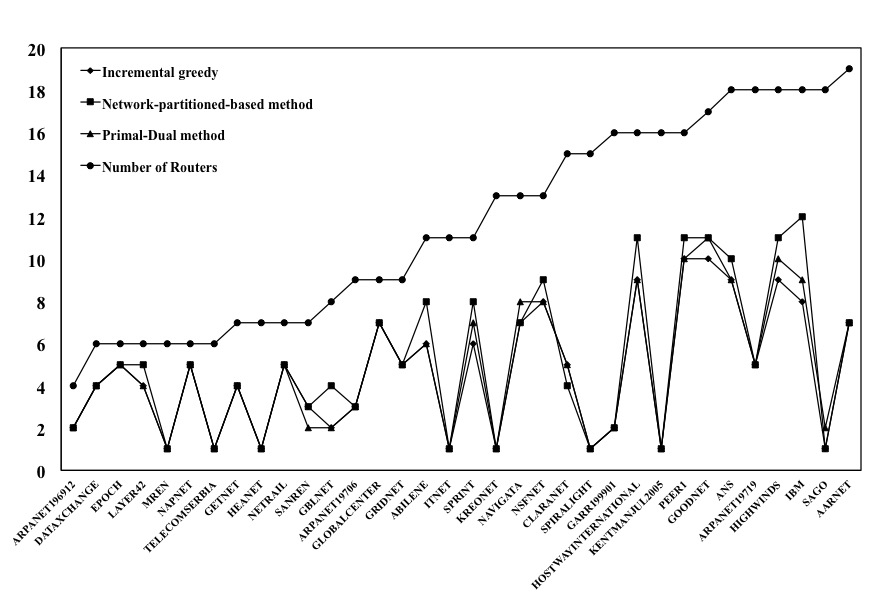
\includegraphics[width=0.50\textwidth]{fig/first.jpg}
\caption{Number of Controllers VS Number of Routers}
\label{fig:results:a}
\end{figure}

\begin{figure}[!htbp]
\center
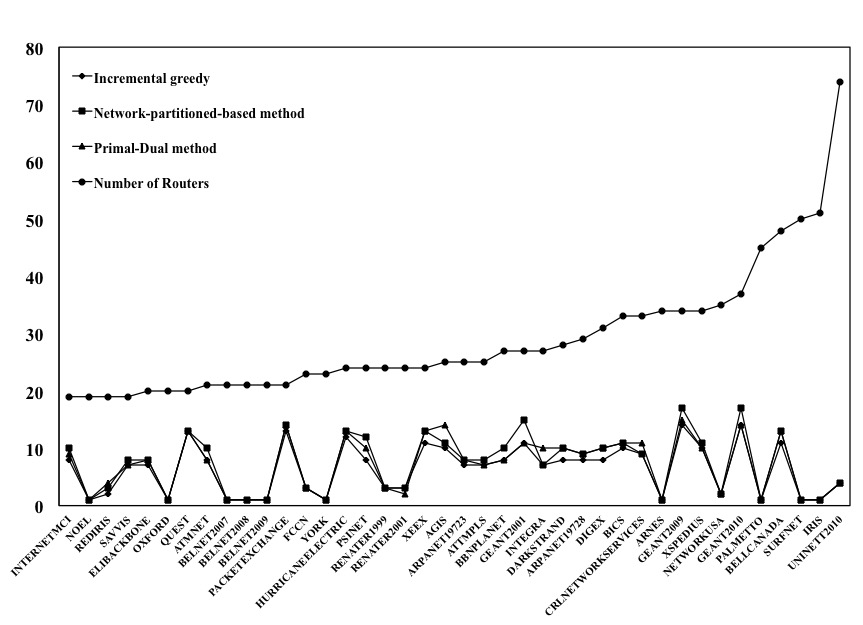
\includegraphics[width=0.48\textwidth]{fig/second.jpg}
\caption{Number of Controllers VS Number of Routers}
\label{fig:results:b}
\end{figure}

\begin{figure}[!htbp]
\center
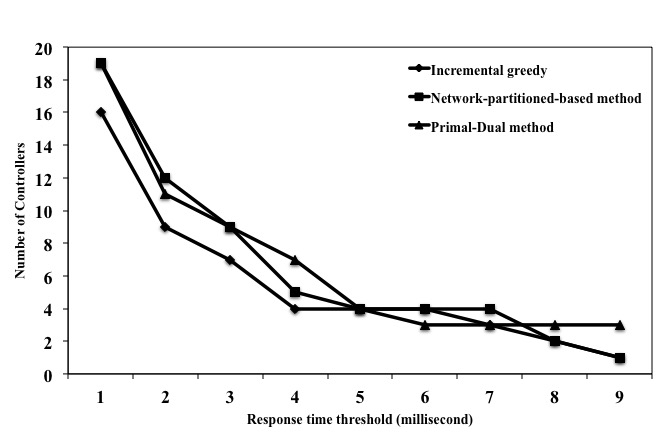
\includegraphics[width=0.48\textwidth]{fig/bound.jpg}
\caption{Comparison results under different value of $\delta$ in one topology}
\label{fig:results:c}
\end{figure}


The three heuristic methods are compared under 74 connected WAN topologies, simulation results are shown in two figures. Figure \ref{fig:results:a} and Figure \ref{fig:results:b} show the number of controllers output by the three methods and the total number of routers of each network topology. The number of routers for each WAN topology ranges from 4 to 74. As it is shown in Figure \ref{fig:results:a} and Figure \ref{fig:results:b}, the number of controllers generated by the three heuristic methods are very close to each other for all input topologies.  

Figure \ref{fig:results:c} shows the performance of the proposed three methods under various value of $\delta$ in one topology. We choose the network topology named UNINETT2010, which has 74 nodes. For this network topology, we compute 9 different value of $\delta$: 1 ms to 9 ms, as it is shown in the X-axis of Figure \ref{fig:results:c}. We can see that the performance of the three methods are very close to each other under various value of $\delta$. From the above three simulation results, we can conclude that the proposed three heuristic methods have the similar performance.

\section{conclusion}
\label{sec:conclusion}
In previous works for controller placement, much concern has been focused on placing $k$ controllers to optimize performance metrics such as propagation latency, load distribution, network reliability. However, in the actual applications, the number of controllers is unknown beforehand. Moreover, the quality of service (QoS) is always a primary concern of the network operators in the placement of SDN controllers. For this reason, we introduce the QoS-Guaranteed Controller Placement problem: Given a network topology and a response time bound, how many controllers need to be instantiated, where they are deployed, and which network nodes are under control of each of the controller, in order to guarantee the response time between a node and its subscribed controller is less than the threshold. We propose three heuristic algorithms to solve this controller placement problem with the required response time constraint. The proposed heuristic methods are compared on the Internet Topology Zoo, a public network topology dataset. The simulation results demonstrate that the proposed three heuristic methods have similar performance on all input topologies.

\bibliographystyle{abbrv}
\bibliography{reference}
\end{document}

